\documentclass{standalone}
\usepackage{tikz}

\begin{document}
  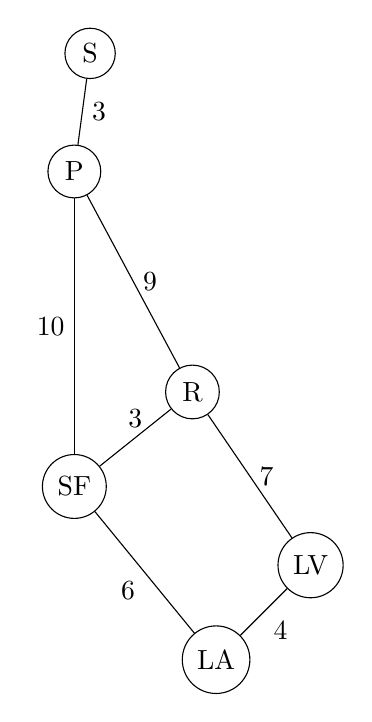
\begin{tikzpicture}
    \node[shape=circle,draw=black] (S) at (-1.8,7.5) {S};
    \node[shape=circle,draw=black] (P) at (-2,6) {P};
    \node[shape=circle,draw=black] (SF) at (-2,2) {SF};
    \node[shape=circle,draw=black] (R) at (-0.5,3.2) {R};
    \node[shape=circle,draw=black] (LA) at (-0.2,-0.2) {LA};
    \node[shape=circle,draw=black] (LV) at (1,1) {LV} ;

    \path (S) edge node [right] {3} (P);
    \path (P) edge node [right] {9} (R);
    \path (P) edge node [left] {10} (SF);
    \path (SF) edge node [above] {3} (R);
    \path (SF) edge node [below left] {6} (LA);
    \path (R) edge node [right] {7} (LV);
    \path (LA) edge node [below right] {4} (LV);
  \end{tikzpicture}
\end{document}
